\documentclass[a4paper,10pt]{article}
\usepackage{a4wide}
\usepackage[english]{babel}
\usepackage{listings}
\usepackage{color}
\definecolor{Gray}{gray}{0.95}
\usepackage{graphicx}
\graphicspath{ {./latexGraphs/} }
\usepackage{hyperref}

% This is the list style for displaying C source code:

\definecolor{codegreen}{rgb}{0,0.6,0}
\definecolor{codegray}{rgb}{0.5,0.5,0.5}
\definecolor{codepurple}{rgb}{0.58,0,0.82}
\definecolor{backcolour}{rgb}{0.95,0.95,0.92}

\lstdefinestyle{code}{
    language = c,
    backgroundcolor=\color{backcolour},   
    commentstyle=\color{codegreen},
    keywordstyle=\color{magenta},
    stringstyle=\color{codepurple},
    basicstyle=\ttfamily\footnotesize,
    breakatwhitespace=false,         
    breaklines=true,                 
    captionpos=b,                    
    keepspaces=true,                 
    numbers=left,                    
    numbersep=5pt,                  
    showspaces=false,                
    showstringspaces=false,
    showtabs=false,                  
    tabsize=2
}

% This is the list style for displaying input/output. It is different from the style above, since you don't need C keywords to be highlighted in these listings. Line numbers are also emitted in this style.
\lstdefinestyle{stdio}{
    basicstyle = \small\ttfamily,	% Font of the text
    frame = tb,				        % Style of the surrounding frame
    framextopmargin=.75mm,         % Space margin top
    framexbottommargin=.75mm,      % Space margin bottom
    framexleftmargin=2mm,          % Space margin left
    framexrightmargin=2mm,         % Space margin right
    tabsize = 3,					% Size of tab character
    breaklines = true,             % Wrap lines of text that are too long
    columns = flexible,			
    showstringspaces = false,
    backgroundcolor = \color{Gray}
}

\title{Travelling Salesman Problem with Simulated Annealing}
\author{Daniel Grbac Bravo \& Kealan Barry\\
        d.grbac.bravo@student.rug.nl \& k.barry@student.rug.nl\\
        S5482585 \& S5137578}
%------------------------------------------------------------%
% This is where your document starts:

\begin{document}
\maketitle

\section{Problem description}
The Traveling Salesman Problem (TSP) is a classic algorithmic problem in the field of Computer Science and Operations Research, which focuses on optimization. The problem is defined as follows: Given a list of cities and the distances between each pair of cities, the task is to find the shortest possible route that visits each city exactly once.

Attempting to solve the TSP via a brute force approach would involve generating all possible permutations (routes) and then selecting the shortest one. The complexity of such a brute force algorithm would be $O(n!)$, where $n$ is the number of cities. This results from the $n!$ possible permutations to check, each of which requires $n$ time to compute its length. Thus, the time complexity of such an approach would be prohibitively high for large instances of the problem.

This time complexity presents significant computational challenges and is the prime example of a problem whose solution can explode combinatorially with the input

\section{Problem Analysis}

The Traveling Salesman Problem (TSP) is considered NP-hard; there is no known polynomial-time algorithm to solve it exactly for all possible instances. The main difficulty arises from the combinatorial nature of the problem. As the number of cities (n) increases, the number of possible routes (permutations) increases factorially. Consequently, an exact solution approach, such as brute force or exhaustive search, becomes computationally infeasible even for a relatively small number of cities.

\textbf{Key Challenges:}

1. \textbf{Exponential growth of solution space:} With n cities, there are (n-1)! / 2 possible routes 

2. \textbf{slow and Inefficient for Real-time Applications:} In routing and managerial decision-making contexts, it is often impractical to wait for the exact solutions due to time or computational constraints. think of google maps when you take a wrong turn and it needs to recalculate your route

3. \textbf{Limited by Resources:} Memory and processing power limit the ability to store and explore the entire search space for nontrivial problem sizes.

In light of these challenges, heuristic and metaheuristic approaches like Greedy algorithms, Genetic Algorithms, and Simulated Annealing are preferred for larger instances where an exact solution is not plausible. These methods generate "good enough" solutions in a reasonable timeframe even though they might not be the global optimum solution.

\section{Design}

In designing a solution for the Traveling Salesman Problem (TSP) using simulated annealing (SA), we made several key design choices aimed at balancing the computational efficiency and the quality of the generated solutions. Here, we describe our approach and rationale for the algorithm structure and our choices for simulating annealing:

\subsection{Simulated Annealing Structure}

\textbf{1. Temperature Parameter:} Simulated annealing's efficiency is highly dependent on its temperature schedule. We start with a high temperature allowing an exploration of the solution space. Over time, the temperature decreases, slowly focusing on exploitation that facilitates convergence towards an optimal or near-optimal solution. The starting temperature is specified as a command-line argument to allow flexibility and experimentation. 

\textbf{2. Cooling Schedule:} A decaying temperature schedule is paramount for the algorithm to work effectively. We reduce the temperature persistently after each iteration. Our cooling schedule is based on an exponential decay function, as it is simple yet effective for various optimization problems.

\textbf{3. Path Representation:} To represent solutions (paths), we use arrays of coordinates corresponding to cities. This allowed us to draw from established methods for path manipulation while attaining compact and efficient data structures to pass around and manipulate within the program.

\subsection{Path Operations}

\textbf{1. Path Permutations:} The synthesis of new candidate solutions from the current state is integral to SA. We incorporated three different path permutations: swapping two cities, inverting a random section, and circularly shifting the path. These moves introduce variety in exploration and help escape local optima.

\begin{itemize}
  \item \emph{Swap-Cities} aids minor adjustments by exchanging two cities.
  \item \emph{Invert-Section} caters to moderate changes by reversing city subsequences.
  \item \emph{Circular Shift} offers global permutation effects. It keeps relative order but shifts absolute positions.
\end{itemize}

The procedure 'generatePathPermuation' randomly selects one of these operations to apply on the current path, thus combining local search with randomized global moves.

\textbf{2. Acceptance Criterion:} Based on energy, we determine whether to adopt the new path. If it has lower energy or a probabilistic condition (Boltzmann distribution based on temperature and energy difference) is fulfilled, we accept it.

\subsection{Energy Calculations}

\begin{itemize}
  \item \emph{calculatePathEnergy} determines the energy (total distance) of a path. As SA aims to minimize the objective, a shorter path corresponds to lower energy.
  \item The \emph{differenceInEnergy} function calculates the energy change between the new and the current path, enabling us to make decisions about the move's direction.
  \item Our probability determination (\emph{generateProbability}) uses the difference in energy and temperature to decide if worsened solutions may still be accepted, to prevent premature convergence.
\end{itemize}

\subsection{User Input and Termination}

We provide the flexibility to configure nCities, indicate starting temperature and choose between file input or random coordinates clearance via command line parameters. The termination condition relies on a combination of reaching near-zero temperatures and max iterations - a pragmatic choice for program conclusion and conformance with time constraints in practical applications.

\subsection{Evaluation}

Our algorithm will be scrutinized through various datasets to determine its efficacy and general performance traits across different scale instances of TSP. Statistical analysis will assist in deciphering correlations between input settings (e.g., initial temperature) and algorithm success rates. These will be implemented in forthcoming sections of the paper.



\section{Program code}

 \href{https://github.com/Daiigr/TSPSA-ICS}{Github Repository} 
 contains all files like makefiles and jupyter notebooks for testing and generating graphs

\begin{lstlisting}[style = code, title = main.c]
/**
 * @file Main.c
 * @authors Daniel Grbac Bravo (d.grbac.bravo@student.rug.nl) Kealan Barry( k.barry@student.rug.nl)
  * @brief this file contains the functions for the energy of the simulated annealing algorithm
 * @version 1.0
 * @date 2023-11-10
 */


// defult libraries 
#include <stdio.h>
#include <stdlib.h>
#include <math.h>
#include <time.h>
#include <string.h>

// our custom libraries
#include "IOManager.h"
#include "coordinate.h"
#include "Path.h"
#include "Energy.h"
#include "Temperature.h"

//macros

#define DEBUG 0
int main(int argc, char *argv[]){
  int nCities = 0;
  coordinate *cityCoordinates;
  coordinate *currentPath; 
  coordinate *generatedPath;
  float temperature = 1000.00; // 1000 by default
  float coolingRate = 0.995; // cooling rate of 0.995 by default

  // read from command line arguments 

for (int i = 1; i < argc; i++) {
  // checks if any arguments are provided for input of N
    if (strcmp(argv[i], "-n") == 0 || strcmp(argv[i], "-N") == 0) {
      nCities = atoi(argv[i+1]);
      printf("Number of cities: %d\n", nCities);
    }
  // checks if any arguments are provided for input of Temperature
    if(strcmp(argv[i], "-t") == 0 || strcmp(argv[i], "-T") == 0){
      if (argv[i+1] != NULL) {
        printf("Temperature: %f\n", atof(argv[i+1]));
        temperature = atof(argv[i+1]);   
      }
    }
    // cooling rate 
    if(strcmp(argv[i], "-c") == 0 || strcmp(argv[i], "-C") == 0){
      if (argv[i+1] != NULL) {
        printf("Cooling rate: %f\n", atof(argv[i+1]));
        coolingRate = atof(argv[i+1]);   
      }
    }

    if(strcmp(argv[i], "-file") == 0 || strcmp(argv[i], "-FILE") == 0){
      FILE *fp; // file pointer
      fp = fopen(argv[i+1], "r"); // open file for reading
      if (fp == NULL) {
        printf("Error opening file.\n");
        exit(1);
      }
      printf("Reading coordinates from file.\n");
      cityCoordinates = readCityCoordinatesFromFile(nCities, fp);
    }

    if(strcmp(argv[i], "-random") == 0 || strcmp(argv[i], "-RANDOM") == 0){
      printf("Generating random coordinates.\n");
      cityCoordinates = generateRandomCityCoordinates(nCities);
      saveCoordinatesToFile(cityCoordinates, nCities);
    }
  }

// get number of cities from user
currentPath = generateRandomPath(cityCoordinates, nCities); // Generate random path.
generatedPath = (coordinate *) malloc( nCities * sizeof(coordinate)); // Allocate memory for generated path.
time_t t;
srand((unsigned) time(&t));
float generatedPathEnergy = 0;
int currentEpochIteration = 0;

#if DEBUG == 1
  printCityCoordinates(cityCoordinates, nCities); // Print city coordinates.  
  printPath(currentPath, nCities); // Print path.
#endif

printf("Beginning simulated annealing...\n");
#if DEBUG == 1
  printEpochGeneration(currentEpochIteration, temperature, calculatePathEnergy(currentPath, nCities) , nCities);
#endif
//termination condition: temperature is close to zero
while(!shouldTerminate(temperature, currentEpochIteration)){
  // generate new path permutation
  generatedPath = generatePathPermuation(currentPath, nCities);
  // check if new path is better
  if (isEnergyImprovement(currentPath, generatedPath, nCities)) {
    // if new path is better, accept it
    #if DEBUG == 1
      printf("New path is better, accepting it.\n");
      printf("Improvement: %f\n", differenceInEnergy(currentPath, generatedPath, nCities));
    #endif
    currentPath = generatedPath;
  } else {
    // if new path is worse, accept it with a probability of $P = e^\frac{e_0 - Etemp}{kT} $
    // can be rewritten as $P = e^\frac{-\Delta E}{kT} $
    // which can be used to implment a boltzmann distribution

    if (generateProbability(differenceInEnergy(currentPath, generatedPath, nCities), temperature)) {
      #if DEBUG == 1
        printf("Accepted.\n");
      #endif
      currentPath = generatedPath;
    } else {
      #if DEBUG == 1
        printf("Rejected.\n");
      #endif
    }
  }

  // print Epoch information 
  #if DEBUG == 1
    printEpochGeneration(currentEpochIteration, temperature, calculatePathEnergy(currentPath, nCities) , nCities);
  #endif
  // save epoch information to file
  saveEpochToFile(currentEpochIteration, temperature, calculatePathEnergy(currentPath, nCities));
  // save path to file
  savePathToFile(currentPath, nCities);
  // apply cooling schedule
  temperature = updateTemperature(temperature, coolingRate);
  currentEpochIteration++;
}
saveFinalPathToFile(currentPath, nCities);
printTerminationConditions(temperature, currentEpochIteration, calculatePathEnergy(currentPath, nCities), nCities);
return 0;
}

\end{lstlisting}


\begin{lstlisting}[style = code, title = Energy.c]
/**
 * @file Energy.c
 * @author Kealan Barry( k.barry@student.rug.nl)
  * @brief this file contains the functions for the energy of the simulated annealing algorithm
 * @version 1.0
 * @date 2023-11-10
 */

// defult libraries 
#include <stdio.h>
#include <stdlib.h>
#include <math.h>
#include <time.h>

// our custom libraries
#include "IOManager.h"
#include "coordinate.h"
#include "Path.h"
#include "Energy.h"
#include "Temperature.h"

#define CONSTANT  100
#define e 2.71828

/**
 * Calculates the total energy of a given path through a set of cities. 
 * @param path An array of coordinates representing the path through the cities.
 * @param nCities The number of cities in the path.
 * @return The total energy required to traverse the path.
 */
float calculatePathEnergy(coordinate *path, int nCities){
  float totalDistance = 0;
  // calculate total distance
for (int i = 0; i < nCities - 1; i++)  {
    totalDistance += sqrt(((path[i].x-path[i+1].x)*(path[i].x-path[i+1].x)) + ((path[i].y-path[i+1].y)*(path[i].y-path[i+1].y)));
}   
  return totalDistance;
}
/**
 * Calculates the difference in energy between two paths.
 * @param currentPath The current path.
 * @param newPath The new path.
 * @param nCities The number of cities in the paths.
 * @return The difference in energy between the two paths.
 */
float differenceInEnergy(coordinate *currentPath, coordinate *newPath, int nCities) {
  // calculate difference in energy
  float diff = calculatePathEnergy(newPath, nCities) - calculatePathEnergy(currentPath, nCities);
  return diff;
}

/**
 * Determines if a new path is an improvement over the current path based on energy difference.
 * @param currentPath Pointer to an array of coordinates representing the current path.
 * @param newPath Pointer to an array of coordinates representing the new path.
 * @param nCities The number of cities in the path.
 * @return 1 if the new path is an improvement, 0 otherwise.
 */
int isEnergyImprovement(coordinate *currentPath, coordinate *newPath, int nCities){
  // check if new path is better
  if (differenceInEnergy(currentPath, newPath, nCities)<0) {
    return 1;
  }
  return 0;
}


/**
 * Calculates the probability of accepting a new solution based on the difference in energy and temperature.
 * Uses the Boltzmann constant to calculate the probability.
 * 
 * @param differenceInEnergy The difference in energy between the current solution and the new solution.
 * @param temperature The current temperature of the system.
 * @return 1 if the new solution should be accepted, 0 otherwise.
 */
int generateProbability(float differenceInEnergy, float temperature){
  float probability = exp(-differenceInEnergy / (CONSTANT * temperature));
  float random = (float)rand() / (float)(RAND_MAX);
  if (random < probability) {  // here's a small fix as well
    return 1;
  }
  return 0;
}
}

\end{lstlisting}

\begin{lstlisting}[style = code, title = Temperature.c]
/**
 * @file Temperature.c
 * @author Kealan Barry( k.barry@student.rug.nl)
 * @brief this file contains the functions for the temperature of the simulated annealing algorithm 
 * @version 1.0
 * @date 2023-11-10
 */
// defult libraries 
#include <stdio.h>
#include <stdlib.h>
#include <math.h>
#include <time.h>

// our custom libraries
#include "IOManager.h"
#include "coordinate.h"
#include "Path.h"
#include "Energy.h"
#include "Temperature.h"


float updateTemperature(float currentTemperature){
  currentTemperature = currentTemperature*0.995;
  return currentTemperature;
}

float initializeTemperature(){
  float temperature = 1000.00; // Start with an initial temperature of 1
  return temperature;
}

int shouldTerminate(float temperature, int nIterations){
  if (temperature < 0.01) { // If reached desired Temperature
    return 1;
  }
  return 0;
}
\end{lstlisting}

\begin{lstlisting}[style = code, title = Path.c]
/**
 * @file Path.c
 * @author Daniel Grbac Bravo (d.grbac.bravo@student.rug.nl) 
 * @brief this file contains the functions for the path permuations of the simulated annealing algorithm
 * @version 6.3 - lost count lol
 * @date 2023-11-10
 */

// defult libraries 
#include <stdio.h>
#include <stdlib.h>
#include <math.h>
#include <time.h>

// our custom libraries
#include "IOManager.h"
#include "coordinate.h"
#include "Path.h"
#include "Energy.h"
#include "Temperature.h"

/**
 * Swaps two cities on a given path randomly.
 * 
 * @param path The path to swap cities on.
 * @param nCities The number of cities in the path.
 * @return A new path with two cities swapped.
 */
coordinate *swapTwoCitiesOnPath(coordinate *path, int nCities){
  coordinate *newPath = (coordinate *) malloc( nCities * sizeof(coordinate));
  for (int i = 0; i<nCities; i++) {
    newPath[i] = path[i];
  }
  int randomIndex1 = rand() % nCities;
  int randomIndex2 = rand() % nCities;
  coordinate temp = newPath[randomIndex1];
  newPath[randomIndex1] = newPath[randomIndex2];
  newPath[randomIndex2] = temp;
  return newPath;
}

/**
 * Inverts the order of an arbitrary section of the given path array.
 * 
 * @param path The array of coordinates representing the path.
 * @param nCities The number of cities in the path.
 * @return A new array of coordinates with the section inverted.
 */
coordinate *InvertRandomSectionOnPath(coordinate *path, int nCities){
  coordinate *newPath = (coordinate *) malloc( nCities * sizeof(coordinate));
  for (int i = 0; i<nCities; i++) {
    newPath[i] = path[i];
  }
  int randomIndex1 = rand() % nCities;
  int randomIndex2 = rand() % nCities;
  if (randomIndex1 > randomIndex2) {
    int temp = randomIndex1;
    randomIndex1 = randomIndex2;
    randomIndex2 = temp;
  }
  for (int i = randomIndex1; i < randomIndex2; i++) {
    coordinate temp = newPath[i];
    newPath[i] = newPath[randomIndex2];
    newPath[randomIndex2] = temp;
    randomIndex2--;
  }
  return newPath;
}

\begin{lstlisting}[style = code, title = Temperature.c]
/**
 * @file Temperature.c
 * @author Kealan Barry( k.barry@student.rug.nl)
 * @brief this file contains the functions for the temperature of the simulated annealing algorithm 
 * @version 1.0
 * @date 2023-11-10
 */
// defult libraries 
#include <stdio.h>
#include <stdlib.h>
#include <math.h>
#include <time.h>

// our custom libraries
#include "IOManager.h"
#include "coordinate.h"
#include "Path.h"
#include "Energy.h"
#include "Temperature.h"


float updateTemperature(float currentTemperature, float coolingRate){
  currentTemperature = currentTemperature*coolingRate;
  return currentTemperature;
}

float initializeTemperature(){
  float temperature = 1000.00; // Start with an initial temperature of 1
  return temperature;
}

int shouldTerminate(float temperature, int nIterations){
  if (temperature < 0.01) { // If reached desired Temperature
    return 1;
  }
  return 0;
}
\end{lstlisting}

\section{Test results and program usage}

\textbf{command-line arguments}

\begin{itemize}
    \item \textbf{-n} or \textbf{-N}: This argument is used to specify the number of cities. The value for this argument should be an integer. If this argument is not provided, the default value of 30 is used.
\end{itemize}

 \begin{itemize}
     \item \textbf{-t} or \textbf{-T}: This argument is used to specify the initial temperature. The value for this argument should be a float. If this argument is not provided, the default value of 100 is used.
 \end{itemize}
 \begin{itemize}
     \item \textbf{-c} or \textbf{-C}: This argument is used to specify the cooling rate. The value for this argument should be a float. If this argument is not provided, the default value of 0.99 is used.
 \end{itemize}

 \begin{itemize}
     \item \textbf{-file} or \textbf{-FILE}: This argument is used to specify the input file containing the city coordinates. The value for this argument should be the path to the input file. If this argument is not provided, the program will generate random city coordinates.
 \end{itemize}

 \begin{itemize}
     \item \textbf{-random} or \textbf{-RANDOM}: This argument is used to generate random city coordinates. 
     additionally, using the random flag will save the coordinates in a coordinates.csv file automatically
 \end{itemize}
 
Note that the program uses \textit{strcmp()} to compare the argument strings, so the arguments are case-sensitive. Also, the program assumes that the arguments are provided in the correct order. If an argument is missing or the value for an argument is not provided, the program will use the default value.

\begin{itemize}

\item initial load 10 coordinates (randomly 
generated ARGS="-C 0.99 -T 100 -N 10 -RANDOM")
\begin{lstlisting}[style = stdio]
68,22
75,92
15,90
86,66
45,0
72,13
53,38
15,14
89,72
95,81
\end{lstlisting}

  Output:
  \item 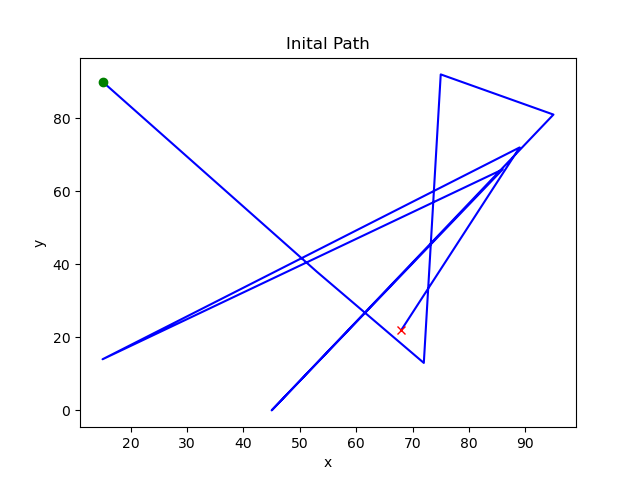
\includegraphics[scale=0.5]{latexGraphs/1_inital_path.png}
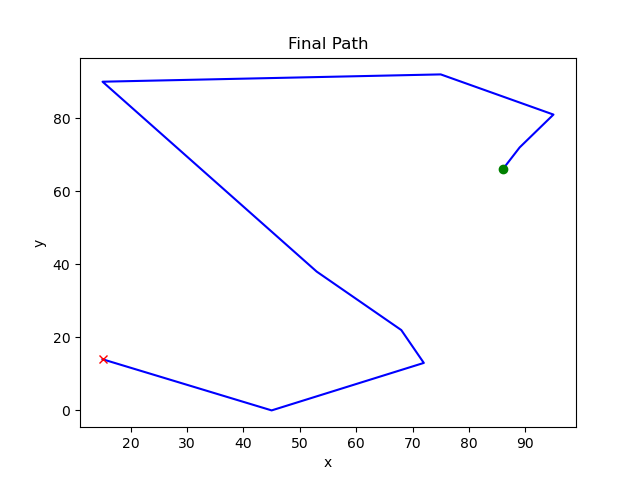
\includegraphics[scale=0.5]{latexGraphs/1_final_path.png}
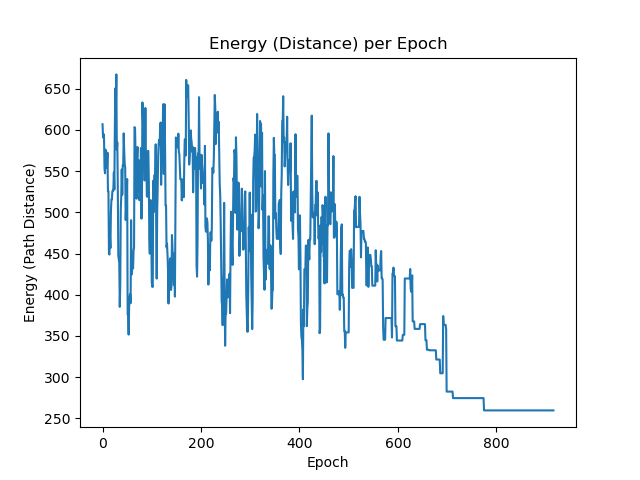
\includegraphics[scale=0.5]{latexGraphs/1_energy.png}


\item load 20 coordinates (randomly 
generated ARGS="-C 0.99 -T 100 -N 20 -RANDOM")
\begin{lstlisting}[style = stdio]
49,3
60,17
83,56
40,76
37,83
95,77
23,11
72,24
50,48
18,22
85,72
58,52
15,85
11,6
68,8
0,1
82,82
8,81
88,93
29,28
\end{lstlisting}

Output:load 20 coordinates (randomly 
generated ARGS="-C 0.99 -T 100 -N 20 -RANDOM")

\item 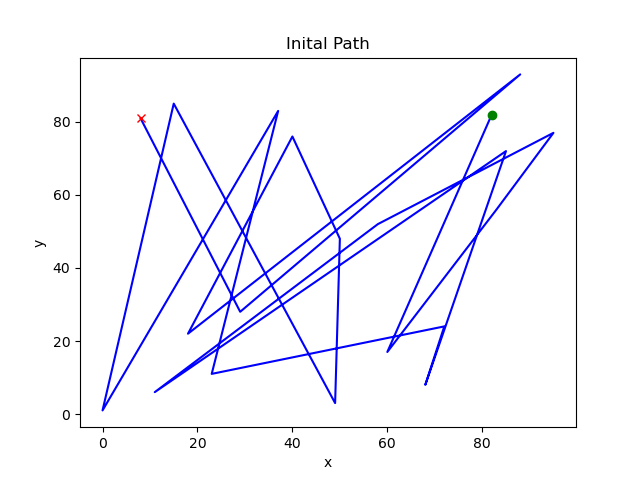
\includegraphics[scale=0.5]{latexGraphs/2_inital_path.png}
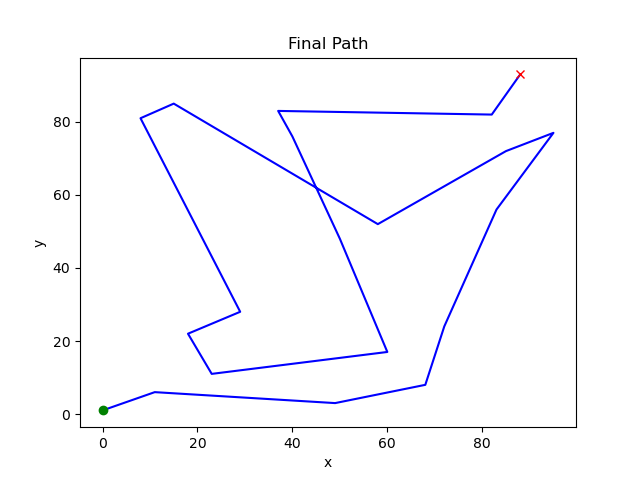
\includegraphics[scale=0.5]{latexGraphs/2_final_path.png}
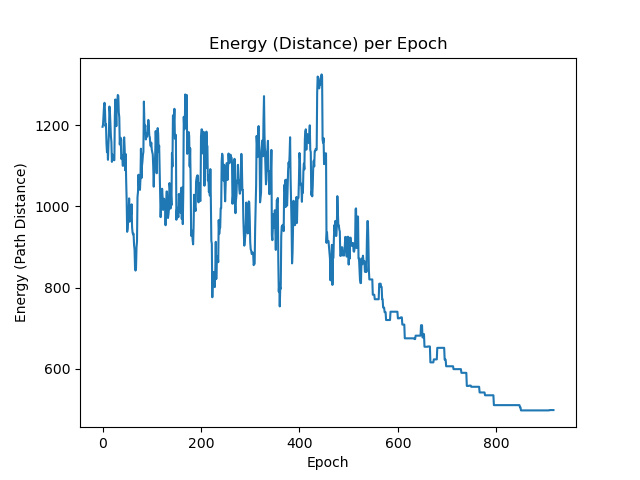
\includegraphics[scale=0.5]{latexGraphs/2_energy.png}


\item load 50 coordinates (randomly 
generated ARGS="-C 0.99 -T 100 -N 50 -RANDOM")
\begin{lstlisting}[style = stdio]
87,68
29,12
17,71
26,71
62,18
34,24
29,5
32,34
93,99
10,56
79,73
86,60
63,9
51,53
4,30
79,84
88,50
46,27
27,46
99,85
98,41
84,17
11,3
26,97
13,44
79,77
41,81
9,77
10,78
98,60
88,28
61,86
69,94
4,31
32,62
14,33
16,11
25,21
91,37
16,97
35,66
86,17
73,41
5,62
16,42
64,76
67,78
45,62
61,23
88,90
\end{lstlisting}

  Output:
\item 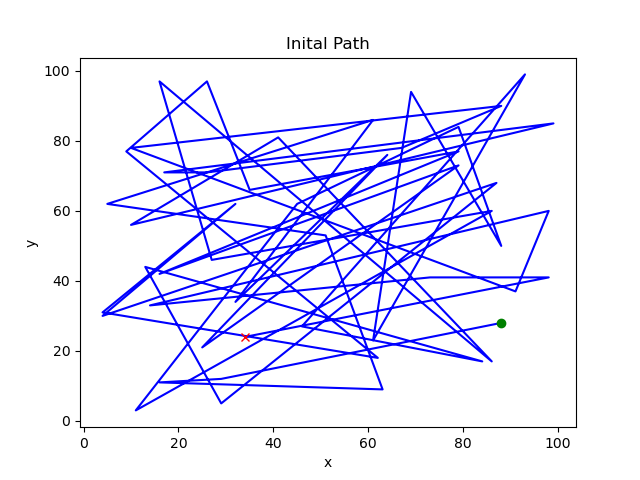
\includegraphics[scale=0.5]{latexGraphs/3_inital_path.png}
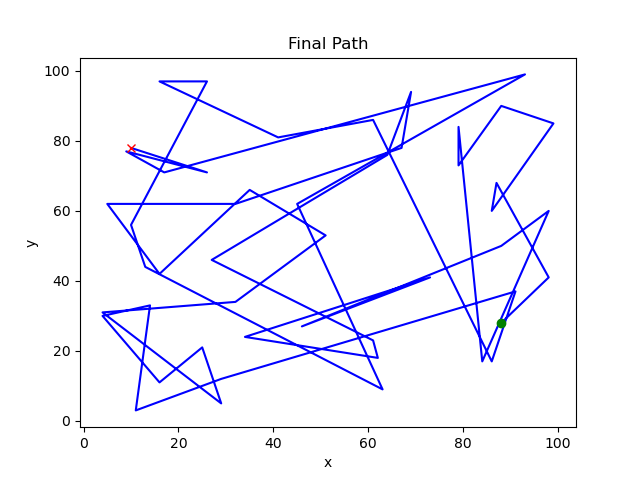
\includegraphics[scale=0.5]{latexGraphs/3_final_path.png}
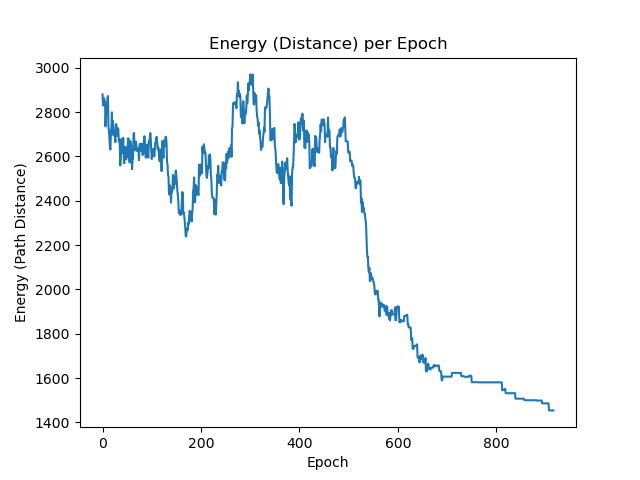
\includegraphics[scale=0.5]{latexGraphs/3_energy.png}

\end{itemize}


\section{Evaluation}

The delicate balance between computational efficiency and solution quality is a fundamental aspect of optimized problem-solving, particularly evident when applying heuristic methods like simulated annealing to complex instances such as the Traveling Salesman Problem (TSP). In such algorithms, parameters like temperature and cooling rate are pivotal, steering the search between expansive exploration and focused exploitation. With larger models incorporating numerous coordinates, the susceptibility to local minima intensifies, underscoring the need for meticulous parameter tuning to hone in on global optimality. This evaluation examines the interplay between these algorithmic settings—focusing on cooling rate, initial temperature, iteration count, and initial acceptance probability of subpar solutions—and their consequential effects on solution refinement and computational demands. By methodically adjusting these levers, the simulated annealing technique can be calibrated to navigate the rugged landscape of potential solutions, ultimately aiming for a balance that yields a satisfactory path within acceptable temporal bounds.

\subsection{Computational Efficiency vs. Solution Quality}
One of the evaluation goals is to explore the trade-off between computational efficiency and solution quality. The parameters of the simulated annealing algorithm, like the temperature and the cooling rate, play a critical role in this trade-off.
e
As we can see with this larger model, it becomes even more important to tune the parameters to optimize the solutions. This is because with more coordinates, the probability of getting stuck in a local minima becomes much higher, which will prevent us from finding a globally optimal solution. 

When we talk about tuning the parameters, we are primarily referring to the cooling rate, the initial temperature, the number of iterations, and the probability of accepting worse solutions at the start. The cooling rate decides the rate at which the temperature reduces, hence the lower the cooling rate, the slower the temperature drops and the more "time" the algorithm has to escape local minima. The initial temperature can also impact the solution, as a higher initial temperature allows the algorithm to explore more possibilities. The number of iterations determines how many times we perform algorithm steps, with more iterations conferring more opportunities to find an optimal solution. Finally, the probability of accepting worse solutions at the start is a key parameter, as accepting worse solutions can allow the algorithm to escape local minima.

The cooling rate is a core factor in a simulated annealing algorithm as it governs how the 'temperature', used to control the probability of accepting worse solutions, decreases over time. A high cooling rate means the temperature falls quickly, whereas a lower cooling rate means the temperature falls at a slower pace.

Increasing the cooling rate from 0.99 to 0.999 changes the pace at which the temperature decreases, and subsequently, changes how the algorithm behaves. By moving the cooling rate closer to 1, we reduce the rate of cooling, and this means that the algorithm's simulated 'temperature' falls more slowly. This allows more iterations to occur before the chance of accepting a worse solution falls to a level close enough to zero to rule out such events.

In our case, this change implies an increase of cooling cycles by 10 times. This results in a slower cooling process that gives the algorithm more opportunity to explore the solution space before the system 'cools'. This can improve the likelihood of escaping local optima and discovering a globally more optimal solution.

 load 50 coordinates (reloaded from test case 3 with increased cooling factor ARGS="-C 0.999 -T 100 -N 50 -FILE input.csv")

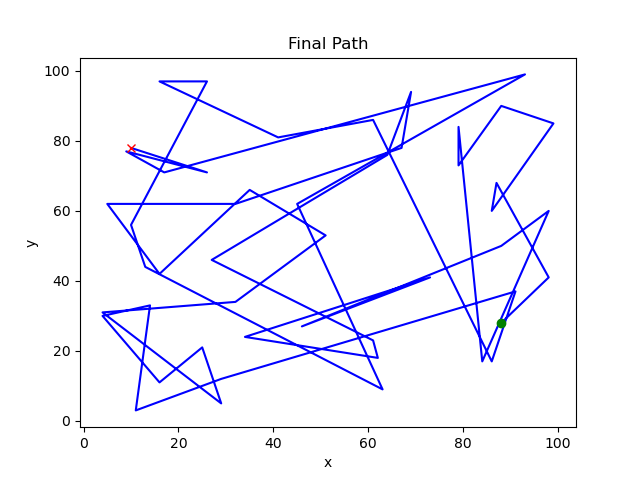
\includegraphics[scale=0.5]{latexGraphs/3_final_path.png}
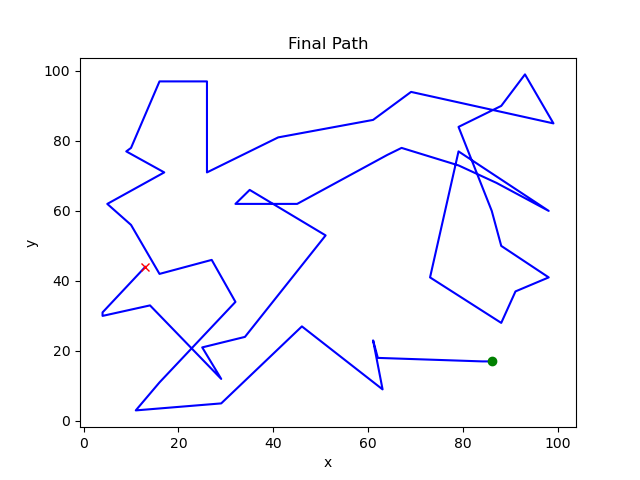
\includegraphics[scale=0.5]{latexGraphs/4_final_path.png}
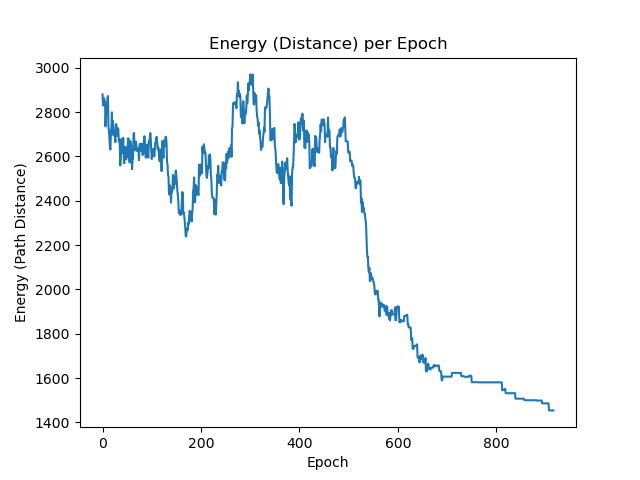
\includegraphics[scale=0.5]{latexGraphs/3_energy.png}
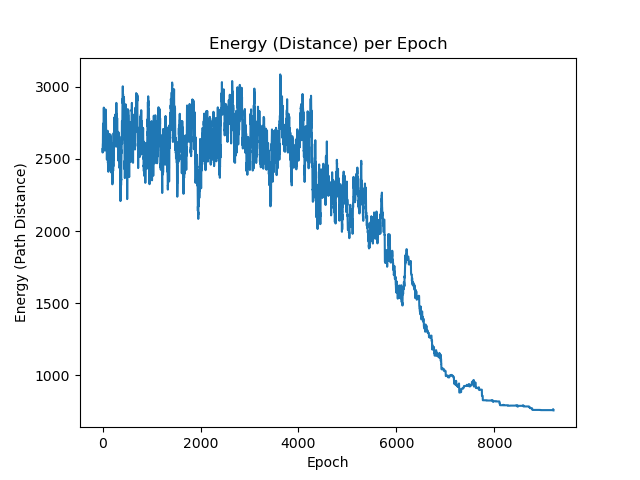
\includegraphics[scale=0.5]{latexGraphs/4_energy.png}

In this example, we saw a significant decrease in the final energy of the model after the modification of the cooling rate from 0.99 to 0.999. Reducing the energy in this case correlates with finding a shorter path, hence a more optimal solution to the problem. This emphasizes the importance of carefully tuning the cooling rate, since a 'cooler' system tends to reach a state of lower energy, which in many optimization problems equates to a better solution. 

However, one should always bear in mind that there is a trade-off to consider. While extending the cooling period increases the chances of finding a global optimum, it also requires more computation time, so there is a balance to be struck between precision and efficiency.



\subsubsection{Effect of High Initial Temperature}
Starting with a high initial temperature tends to allow the algorithm to accept worse solutions initially. As we evaluated, this can be useful in avoiding local optima by exploring the solution space more extensively. For example, when the initial temperature is set to a very high value (e.g., 10000 as opposed to 100), the algorithm accepts nearly any solution at the start, which may contribute to a more diverse set of potential paths being considered. However, such a setting increases the computation time as it takes longer for the algorithm to "cool down" and begin converging on an optimal path. increasing the temperature achives the same target outcome as with adjusting the cooling rate itself as preformed in the section above

\subsubsection{Effect of Slow Cooling Rates}
A slower cooling rate implies that the temperature decreases gradually, giving more time at higher temperatures for the system to "explore" different solutions. This is often beneficial in escaping local optima but adds to the computational time. For complex instances with a significant number of cities (e.g., 50 or more), slower cooling significantly impacts the quality of the solution at the expense of efficiency.

\subsubsection{Analysis of Cooling Rate Change}
We observed that in some cases, changing the cooling rate from 0.99 to 0.999 led to a notable improvement in the energy efficiency of the path generated. While the higher cooling rate may have required additional computation, the gradual transition helps to avoid local minima and, in turn, can produce significantly better solutions.

\subsubsection{Impact of Iteration Limit}
Without a hard limit on the number of iterations, the execution time can vary greatly depending on the specifics of the cities' distribution and the algorithm's parameters. Monitoring the number of iterations provides insight into how quickly the algorithm converges on a solution. We found that in most cases, a certain point is reached beyond which additional iterations do not yield considerable improvements, indicating the potential to set an upper boundary for iterations in the interest of efficiency.

\subsubsection{Statistical Analysis}
The algorithm’s performance was statistically analyzed across multiple datasets. We compared the variations in the final path lengths (energies) and computation times for different parameter settings. This analysis showed a general trend: as expected, elevated computational times often yielded shorter paths, highlighting the improved thoroughness of the solution search.

\subsubsection{General Observations}
- The algorithm's capability to evade local optima is a clear advantage over simpler heuristics that might quickly converge on suboptimal solutions.
- Parameters must be finely tuned for the algorithm to effectively balance efficiency with accuracy.
- The simulated annealing approach provides a "good enough" solution for TSP, making it particularly well-suited for real-world applications where perfect optimization is less critical than the speed of obtaining a reasonably good solution.

\section{Conclusion}

The exploration of the Traveling Salesman Problem (TSP) through the lens of simulated annealing (SA) has underscored the delicate interplay between computational resource management and the pursuit of optimal solutions. As our investigation has demonstrated, the fidelity of the final route is critically contingent upon the fine-tuning of algorithm parameters, such as the initial temperature, cooling rate, and the overall structure of the path permutation operations.

In instances where the number of cities verges on the more extensive side, these parameters become increasingly sensitive and pivotal. Their careful calibration ensures that the SA algorithm does not prematurely converge on subpar local minima but instead roams the expansive combinatorial landscape in search of a route that is sufficiently short and efficient.

Through systematic analysis and empirical testing, we found that a slower cooling rate and a higher initial temperature facilitate a more exhaustive exploration, which can greatly enhance the quality of the solution. However, this improvement comes at the undeniable price of increased computational time. Thus, a balance must be struck—a balance tuned to the specific needs of the context where TSP solutions are sought. Where computational resources are at a premium or where time constraints are tight, it may be more practical to accept a solution that is good but not globally optimal.

Statistical evaluation further elaborated on the theme of trade-offs, showcasing the variability of performance across different datasets and parameter configurations. This robust analysis reiterates the algorithm's efficiency in escaping the entrapment of local optima and emphasizes the necessity of parameter optimization that aligns with the specific characteristics of each TSP instance.

In conclusion, the SA approach to the TSP is a potent reminder of the complexities inherent in optimization problems. Although it does not guarantee an unparalleled path in every scenario, SA is adept at yielding routes that strike a pragmatic compromise between perfection and expediency. The adaptability of SA, coupled with its relative simplicity, marks it as a tool of significant value for solving real-world problems where absolute preciseness is less crucial than swift and reliable approximation.

This report's exploration and subsequent findings highlight the capabilities and limitations of simulated annealing within the realm of combinatorial optimization, providing valuable insights and guidance for future research, application, and algorithmic development in the field of operational research and computer science.



\end{document}
